\chapter{Open Questions and Further Research}\label{ch:closing}

\vspace*{-50pt}

\begin{figure}[ht]
        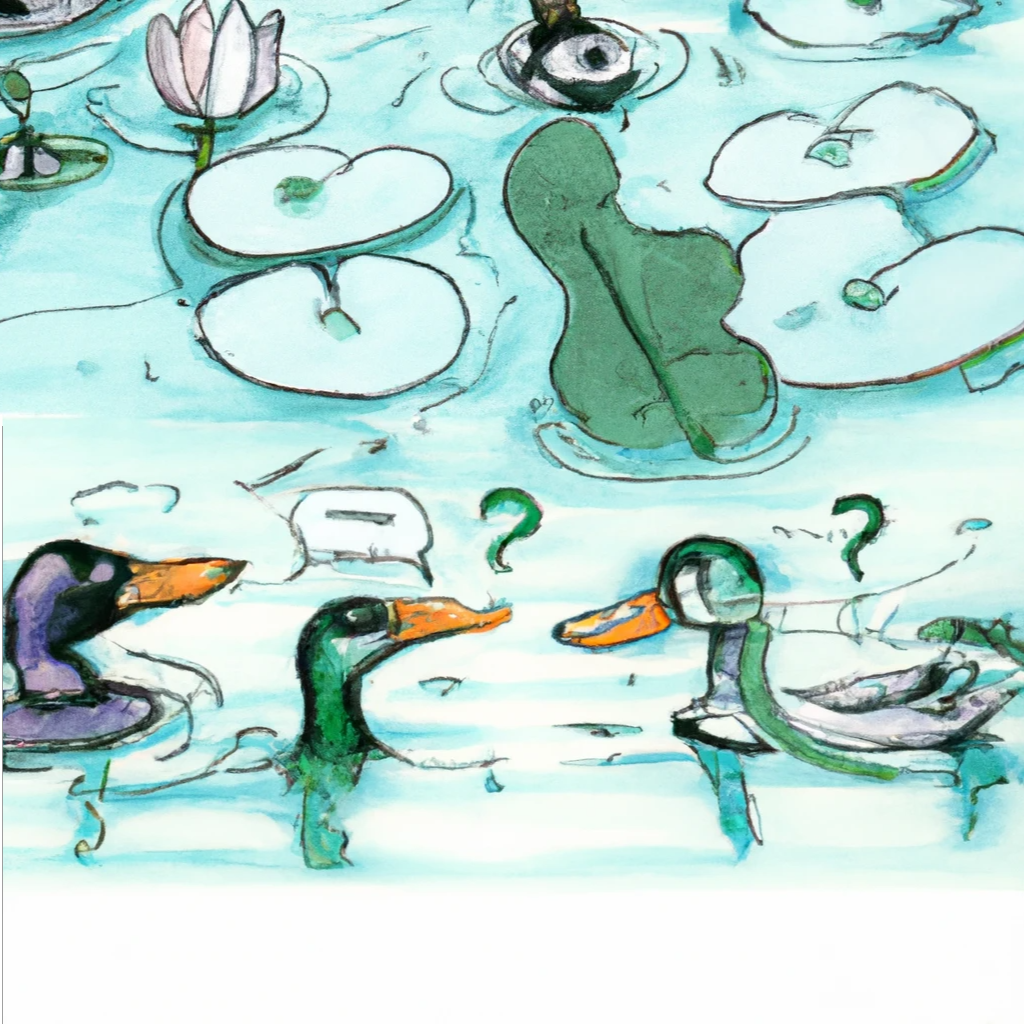
\includegraphics[width=0.35\textwidth, right]{img/further-questions.png}
        \captionsetup{textformat=empty,labelformat=blank}
        \caption{Generated with Dall-E. \url{https://labs.openai.com/}. ``more ducks asking further questions and research topics''}
\end{figure}

\epigraph{\itshape Todo select another quote}{Lewis Caroll, \textit{XXXX}}

* Chordal Bipartite Grap hs a very interesting case.
* Improve the Kernel Bound

Further fpt algorithms especially for classes where \sdom and \tdom already have fpt 

Worst case reduction proven, but what about real / random graphs? How much is the graph being reduced by firing these reduction rules.

Some classical complexities unresolved: dually chordal and tolerance graphs